\documentclass{beamer}
\usetheme{Frankfurt}

\usepackage{listings}

\newcommand{\todo}[1]{\alert{TODO #1}}

\title{Public key encryption/Authentication}
\subtitle{Lecture 4 \\ Computer Security DD2395}
\author[R. Guanciale]{
  Roberto Guanciale\\
  robertog@kth.se
}
\date{2015-11-10}
\begin{document}

\begin{frame}[plain]
  \titlepage
\end{frame}

\begin{frame}{Outline for Today}
  \begin{itemize}
    \item Public key encryption
    \item Authentication
  \end{itemize}
\end{frame}

\begin{frame}{Offtopic}
  \begin{itemize}
    \item $C = (P \oplus K_1) + K_2$
    \item Lab W
  \end{itemize}
\end{frame}

\begin{frame}{Public key encryption}
  \begin{itemize}
    \item Sharing symmetric keys is difficult
    \item No public key  encryption mechanism existed before 1970s
  \end{itemize}
\end{frame}

\begin{frame}{Public key encryption}
  \begin{center}
    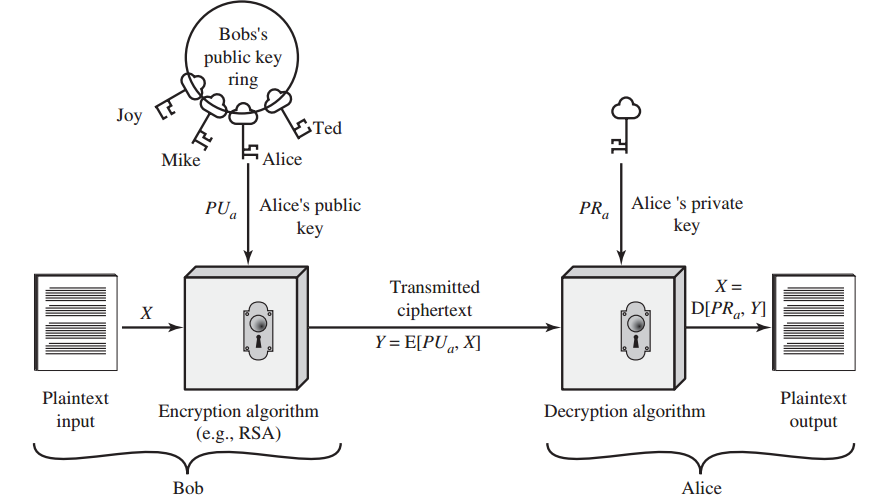
\includegraphics[width=0.8\linewidth]{public1}\\
    Confidentiality
  \end{center}
\end{frame}

\begin{frame}{Public key encryption}
  \begin{center}
    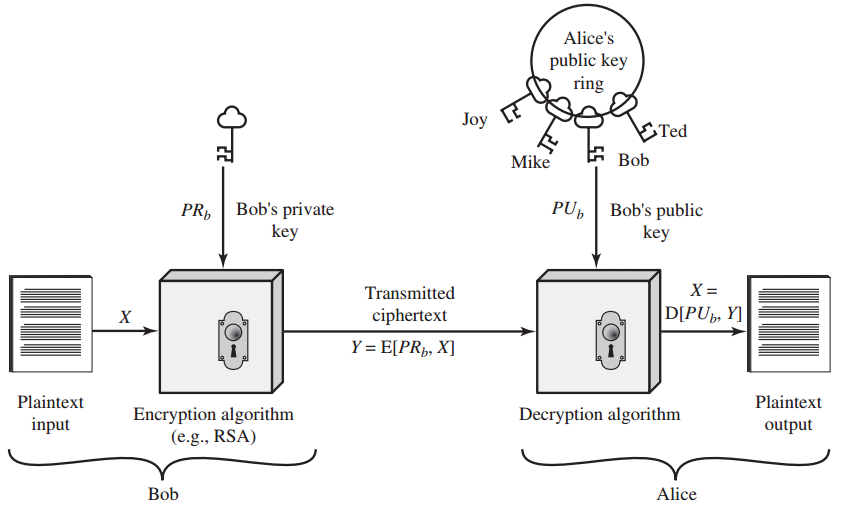
\includegraphics[width=0.8\linewidth]{public2}\\
  Integrity/authentication
  \end{center}
\end{frame}


\begin{frame}{Requirements}
  \begin{itemize}
    \item It is easy for $B$ to generate the key pair $(PU_b,PR_b)$
    \item It is easy for $A$, knowing $PU_b$ and $M$, to compute $C=E(PU_b, M)$ 
    \item It is easy for $B$, knowing $PR_b$ and $C$, to compute $M=D(PR_b, C)$ 
    \item It is not feasible to compute $PR_b$ knowing $PU_b$ 
    \item It is not feasible to infer $M$ knowing $PU_b$ and $C$
    \item (optional) $M=D(PU_b,E(PR_b,M))=D(PR_b,E(PU_b,M))$
  \end{itemize}
\end{frame}
 

\begin{frame}{Applications}
  \begin{center}
    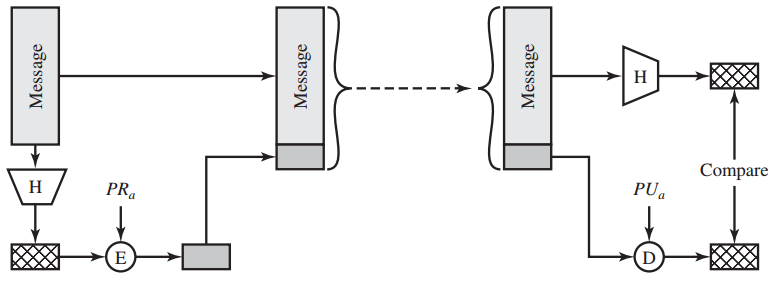
\includegraphics[width=0.8\linewidth]{signature}\\
  Digital Signature (i.e. authentication of sender/integrity of payload)
  \end{center}
\end{frame}
 
\begin{frame}{Applications}
  \begin{center}
    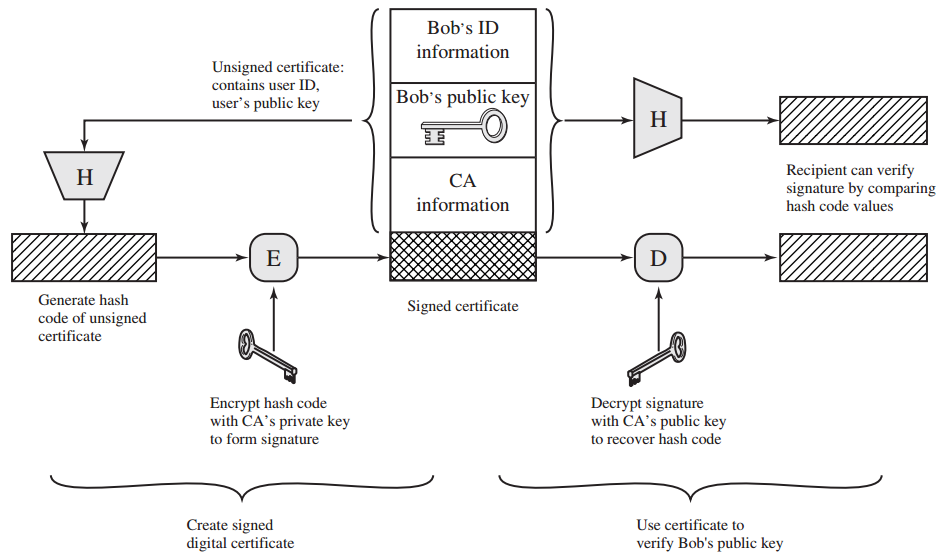
\includegraphics[width=0.8\linewidth]{certificate}\\
  Digital Certificate (i.e. authentication/integrity of public keys)
  \end{center}
\end{frame}

\begin{frame}{Applications}
  \begin{center}
    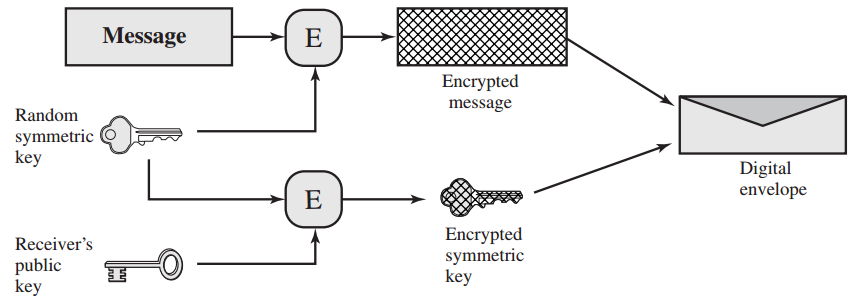
\includegraphics[width=0.8\linewidth]{envelope}\\
  Exchange of symmetric keys/Digital envelopes
  \end{center}
\end{frame}


\begin{frame}{ Ron Rivest, Adi Shamir, and Len Adleman: RSA }
  \begin{itemize}
    \item Encryption: $C = M^e\ mod\ n$
    \item Decryption: $M = C^d\ mod\ n = (M^e\ mod\ n)^d\ mod\ n = (M^e)^d\ mod\ n = M^{ed}\ mod\ n$
    \item $e,d,n$ such that $M = M^{ed}\ mod\ n$
    \item It is easy to compute $M^e\ mod\ n$ and $C^d\ mod\ n$
    \item It is not feasible to discover $d$ knowing $e$ and $n$
  \end{itemize}
\end{frame}

\begin{frame}[t]{Requirement 2: It is easy to compute $M^e\ mod\ n$ and $C^d\ mod\ n$}
  \begin{itemize}
  \item Naive approach: compute $M^e$ ($O(e)$ multiplications, memory intensive)
    
\only<2>{
    \item Memory efficient: $a*b\ mod\ n = (a\ mod\ n)*(b\ mod\ n)\ mod\ n$\\ 
      $e=0$: $c_0 = 0 * M\ mod\ n$\\
      $e=1$: $c_1 = c_0 * M\ mod\ n$\\
      $e=2$: $c_2 = c_1 * M\ mod\ n$\\
      \dots
      $O(e)$ multiplications
      }
    \item<3-> Right to left binary : $e = \prod_i a_i*2^i$\\ 
      thus $M^e = M^{\prod_i a_i*2^i} = \prod_i (M^{2^i})^{a_i}$\\
      thus $M^e\ mod\ n = (\prod_i (M^{2^i})^{a_i})\ mod\ n$\\[20pt]
      $C:=1$\\
      for $i \in [0\dots bits]$\\
      \ \ \ \  if ($a_i=1$) then $C:= C * M\ mod\ n$\\
      \ \ \ \  $M:= M*M\ mod\ n$
  \end{itemize}
\end{frame}

\begin{frame}{Requirement 1: $M = M^{ed}\ mod\ n$}
  \begin{itemize}
    \item<2-> Use $n=p*q$, where $p,q$ primes 
    \item<3-> Let $e$ and $d$ be multiplicative inverse modulo $\phi(n)$ (Euler totient function)
      \begin{itemize}
      \item<4-> $e*d\ mod\ \phi(n) = 1$
      \item<5-> $e*d = 1 + h(\phi(n))$
      \end{itemize}
    \item<6-> assuming that $m$ and $n$ are coprime:
      \begin{itemize}
      \item<7-> Euler theorem: $m^{\phi(n)} \equiv_{mod\ n} 1$
      \item<8-> $m^{ed} $
        \only<9->{$= m^{1 + h(\phi(n))}$}
        \only<10->{$= m*(m^{\phi(n)})^h$}
        \only<11->{$\equiv_{mod\ n} m * 1^h$}
        \only<12->{$\equiv_{mod\ n} m$}
      \end{itemize}
    \item<13> if $m$ and $n$ are not coprime, $m \equiv_{mod\ p} 0$\\
    proof uses Fermat's little theorem
  \end{itemize}
\end{frame}

\begin{frame}{Requirement 1: $M = M^{ed}\ mod\ n$}
  \begin{itemize}
    \item $n=p*q$, where $p,q$ primes 
    \item $e*d\ mod\ \phi(n) = 1$
    \item<2-> Euler total function is multiplicative: $a,b$ coprime then $\phi(a*b) = \phi(a)*\phi(b)$
    \item<3-> If $a$ prime then $\phi(a) = (a-1)$ 
    \item<4-> $\phi(n) = (p-1)(q-1)$
  \end{itemize}
\end{frame}

\begin{frame}{Requirement 1: $M = M^{ed}\ mod\ n$}
  \begin{itemize}
    \item $n=p*q$, where $p,q$ primes 
    \item $e*d\ mod\ \phi(n) = 1$
    \item $\phi(n) = (p-1)(q-1)$
    \item<2-> The multiplicative inverse of $e$ modulo $\phi(n)$ exists if and only if $e$ and $\phi(n)$ are coprime
    \item<3-> Select $e$ as random coprime of $\phi(n)$
    \item<4-> Compute $d$
  \end{itemize}
\end{frame}

\begin{frame}{RSA}
  \begin{itemize}
    \item $n=p*q$, where $p,q$ primes 
    \item $e*d\ mod\ \phi(n) = 1$
    \item $\phi(n) = (p-1)(q-1)$
    \item Select $e$ as random coprime of $\phi(n)$
    \item Compute $d$
    \item $PU = [n,e]$ 
    \item $PR = [n,d]$
    \item Encryption $C = M^e\ mod\ n$
    \item Decryption $D = C^d\ mod\ n$
  \end{itemize}
\end{frame}

\begin{frame}{RSA: security}
  \begin{itemize}
    \item Brute force 
    \item Side channels: e.g. time to decrypt
    \item Mathematical attacks: factorize the product of two prime numbers
  \end{itemize}
  \begin{center}
    \begin{tabular}{|r|r|r|}
      \hline\\
  Number of Decimal Digits &
  Date Achieved & MIPS-Years\\
  \hline
 100 & April 1991 & 7 \\ 
 110 & April 1992 & 75\\
 120 & June 1993 & 830\\
 129 & April 1994 & 5000\\
 130 & April 1996 & 1000\\
 140 & February 1999 & 2000\\
 155 & August 1999 & 8000\\
 \hline
 \end{tabular}
  \end{center}
\end{frame}


\begin{frame}{Other public-key encryption mechanism}
  \begin{itemize}
    \item Dffie-Hellman: generation of a shared symmetric key 
    \item Elliptic curve: like RSA (cheaper, different mathematical assumption)
  \end{itemize}
\end{frame}

\begin{frame}{Stream cyphers}
  \begin{center}
    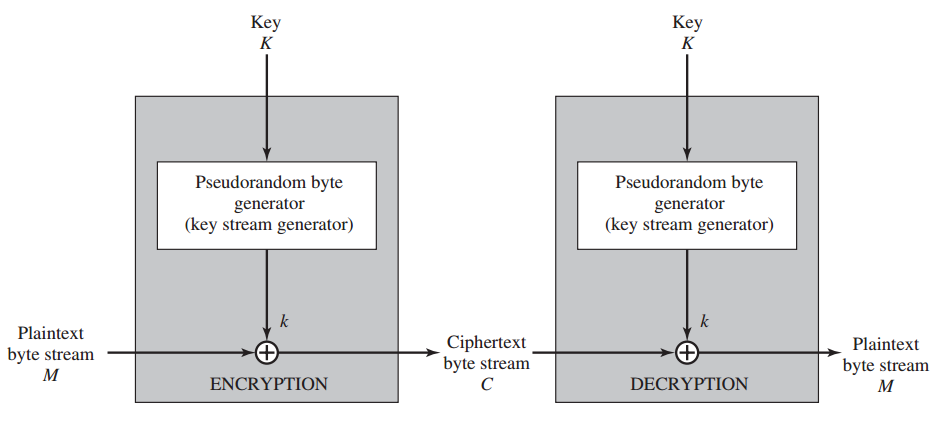
\includegraphics[width=0.8\linewidth]{stream}
  \end{center}
  \begin{itemize}
    \item  encryption sequence should have a large period 
    \item  key stream should resemble a random stream
  \end{itemize}
\end{frame}

\begin{frame}{Authentication}
  \begin{itemize}
    \item Identification step: present an identifier (I'm Roberto, My person number is 19 \dots) 
    \item Verification step: corroborate the binder between the entity and the identifier (that's is my password)
  \end{itemize}
\end{frame}

\begin{frame}{Means of Authentication}
  \begin{itemize}
    \item Something the individual knows (PIN, password, name of the individual's pet) 
    \item Something the individual possesses (physical keys, electronic keycards)
    \item Something the individual is (fingerprint, retina, PUFs)
    \item Something the individual does (voice recognition, handwriting, captcha)
  \end{itemize}
\end{frame}


\begin{frame}{Password based authentication}
  \begin{itemize}
    \item The wider adopted mechanism 
    \item Vulnerability
      \begin{itemize}
        \item Brute force attack (countermeasures: timeout, max errors)
        \item Popular password attack (against several users) (countermeasures: reject password 123123, names, dictionary)
        \item Password guessing attack (against single user) (countermeasures: reject dates)
        \item Workstation hijacking (countermeasures: automatic log-out)
        \item User mistake (writing down the password, phishing)
        \item Multiple password use
        \item Electronic monitoring 
        \item Dependent on how we store the passwords 
      \end{itemize}
  \end{itemize}
\end{frame}

\begin{frame}{Password management}
  \begin{itemize}
    \item Password stored in plaintext: $rec = ID \mid PWD$
    \item Authentication: $PWD = rec.PWD$
      \begin{itemize}
        \item<2-> vulnerable to insider attacks: Sysadmin can read all the passwords
        \item<3-> vulnerable to leakage of the password file (i.e. every 6 months the pwd files of
          Adobe, Sony, \dots is leaked)
      \end{itemize}
  \end{itemize}
\end{frame}

\begin{frame}{Password management}
  \begin{itemize}
    \item Password stored as hashes: $ID \mid HPWD$ where $HPWD=H(PWD)$ 
    \item Authentication: $H(PWD) = rec.HPWD$
      \begin{itemize}
        \item<1-> vulnerable to repetition: if $rec.PWD = rec'.PWD$ then $rec.HPWD = rec'.HPWD$
        \item<2-> vulnerable to collisions: $H(PWD')=H(PWD)$
        \item<3-> Reverse look up tables $L: h \rightarrow pwd$ (only for the most common passwords)
        \item<4-> Cryptanalysis (the most common password in the file is either 123456, password, 12345, 12345678 or qwerty)
        \item<5-> 6 million user-generated passwords; the 10,000 most common passwords give access to 98 percent of all accounts. 
      \end{itemize}
  \end{itemize}
\end{frame}


\begin{frame}{Lookup tables}
  \begin{itemize}
    \item Data: 16 bytes, hash 16 bytes: $2^{128}*16*2$ bytes 
    \item Data: 16 letters, hash 16 bytes: $2^{75}*16*2$ bytes
    \item Data: 16 capital letters, lower letters, digits, hash 16 bytes: $2^{95}*16*2$ bytes
    \item Data: 8 ANSI chars, hash 16 bytes: $2^{56}*16*2$ bytes
    \item Data: English dictionary, hash 16 bytes: $2^{18}*16*2$ bytes
  \end{itemize}
\end{frame}

\begin{frame}{Rainbow tables: compute the inverse of h}
  \begin{itemize}
    \item offline
      \begin{itemize}
      \item let $\mathcal{P}$ be the plaintext space and $\mathcal{H}$ the hash code space
      \item<2-> $H:\mathcal{P} \rightarrow \mathcal{H}$
      \item<3-> define a reduction function $R: \mathcal{H} \rightarrow \mathcal{P}$ (it is not the inverse)
      \item<4-> fix $k$, pick a random subset $\{p_0, \dots, p_n\}$ of $\mathcal{P}$
      \item<5-> compute the chains $p_0$, $h^0_0 = H(p_0)$, $p^1_0 = R(h^0_0)$, $h^1_0 = H(p^1_0)$, \dots, 
        $p^k_0 = R(h^{k-1}_0)$
      \item<6-> store $(p_i, p^k_i)$
      \end{itemize}
    \item online
      \begin{itemize}
      \item<7-> compute the chains $p^1=R(h)$, $h^1 = H(p^1)$, $p^2 = R(h^1)$ \dots
      \item<8-> if $p^n$ is matched by $(p_i, p^k_i)$ 
      \item<9-> recompute the chain of $(p_i, p^k_i)$; if the chain contains $h^j = h$ then $p^j$ is the inverse of $h$
      \end{itemize}
  \end{itemize}
\end{frame}


\begin{frame}{Password management}
  \begin{itemize}
    \item Password salted and hashed: $ID \mid salt \mid HPWD$ where $HPWD=H(PWD, salt)$ 
    \item Authentication: $H(PWD, salt) = rec.HPWD$
  \end{itemize}
\end{frame}

\begin{frame}{Password Selection Strategies }
  \begin{itemize}
    \item User education 
    \item Computer generated password (trust in the algorithm and implementation, hard to remember)
    \item Reactive password checking (periodically run the password cracker to find guessable passwords)
    \item Proactive password checking (online)
      \begin{itemize}
        \item at least eight characters long
        \item must include at least one each of uppercase, lowercase, numeric digits, and punctuation marks
      \end{itemize}
    \item Need of simple datastructures to represent huge dictionaries (e.g. Bloom filters) 
  \end{itemize}
\end{frame}

\begin{frame}{Token based authentication}
  \begin{itemize}
    \item Magnetic card, Smartcard, NFC, SIM card 
    \item Static: user authenticates himself or herself
      to the token and then the token authenticates the user to the computer.
    \item Dynamic password generator: the token generates a unique
      password periodically (e.g., every minute).
    \item Challenge-response: the computer system generates a challenge,
      such as a random string, the token generates a
      response based on the challenge.
  \end{itemize}
\end{frame}

\begin{frame}{Biometric authentication}
  \begin{itemize}
    \item Facial characteristics, Fingerprints, Hand geometry, Iris, Signature, Voice 
    \item Both identification and verification
    \item Verification requires trusted path from the sensor to the checking system
    \item False positive vs False negative
  \end{itemize}
\end{frame}

\begin{frame}{Remote authentication: e.g. password}
  \begin{itemize}
    \item User $U$ wants to authenticate on server $S$
    \item<2-> $U \rightarrow S: PWD$
    \item<3-> $U \rightarrow S: H(PWD)$
    \item<4-> $U \rightarrow S: H(PWD,salt)$
  \end{itemize}
\end{frame}

\begin{frame}{Remote authentication: e.g. password}
  \begin{itemize}
    \item<2-> $U \rightarrow S: id$
    \item<2-> $S \rightarrow U: r, h, f$, where $r$ is a random ``nonce'', $f$ is a function and $h$ is a hash function 
    \item<2-> $U \rightarrow S: v = f(r, h(P))$, where $P$ is the password
    \item<2-> $S$ checks $f(r, h(P\ of\ id)) = v$
    \item<4-> The system stores the hash of the passwords
    \item<5-> Neither the password or its hash code are transmitted, a function that depends on them is transmitted
    \item<6-> The random nonce defends against replay attacks
    \item<2-> Can also be applied to tokens
  \end{itemize}
\end{frame}

\begin{frame}{Security issues}
  \begin{itemize}
    \item Client attacks
    \item Host attacks
    \item Eavesdropping
    \item Replay
    \item Trojan horse
    \item<2> Denial of service
  \end{itemize}
\end{frame}


\begin{frame}{Possible topics for the last lecture}
  \begin{itemize}
    \item Side channel attacks
    \item Secure multiparty computations
  \end{itemize}
\end{frame}

\begin{frame}{Side channel attacks}
      $C:=1$\\
      for $i \in [0\dots bits]$\\
      \ \ \ \ if ($a_i=1$) then $C:= C * M\ mod\ n$\\
      \ \ \ \ $M:= M*M\ mod\ n$
\end{frame}


\begin{frame}{SMC}
  \begin{itemize}
      \item $A$ knows $x$
      \item $B$ knows $y$
      \item $C$ knows $z$
      \item Allow $A$ to obtain $f(x,y,z)$
        \begin{itemize}
          \item without trusted third party
          \item without compromising secrecy
        \end{itemize}
  \end{itemize}
\end{frame}

\end{document}
